\section{Metodologia}

Foi adotada uma abordagem quantitativa, experimental e comparativa. O fator servidor possui dois níveis (Nginx-RTMP e SRS), o fator transcodificador possui dois níveis (FFmpeg e GStreamer) e a carga possui três níveis (1, 10 e 50 espectadores sintéticos). O delineamento fatorial $2\times2\times3$ resulta em 12 tratamentos, cada um repetido três vezes, totalizando 36 execuções. A unidade experimental é uma sessão completa de publicação, transcodificação e leitura HLS executada em um ambiente reconstruído pelo Docker Compose.

\begin{table}[H]
\centering
\caption{Fatores e níveis do experimento}
\begin{tabularx}{\textwidth}{@{}lXX@{}}
\toprule
Fator & Níveis & Papel no experimento \\
\midrule
Servidor RTMP & Nginx-RTMP; SRS & Recebe a publicação RTMP e dispara o processamento \\
Transcodificador & FFmpeg; GStreamer & Gera as variantes HLS \\
Carga & 1; 10; 50 viewers & Simula demanda crescente de leitura \\
Repetição & 3 por tratamento & Permite estimar média e desvio padrão \\
\bottomrule
\end{tabularx}
\end{table}

\subsection{Arquitetura e fluxo experimental}

No benchmark, uma fonte sintética é gerada pelo container \texttt{jrottenberg/ffmpeg:6.0-alpine} com o padrão \texttt{testsrc} em 1280$\times$720 a 30 quadros por segundo, acompanhada por um sinal de áudio senoidal. O publicador envia essa fonte por RTMP ao servidor selecionado. Nginx-RTMP ou SRS aciona o script do transcodificador, que lê o fluxo RTMP, codifica quatro variantes e grava playlists e segmentos HLS. Os viewers sintéticos são containers \texttt{curlimages/curl:8.7.1}; cada um requisita a playlist mestre, uma playlist de variante e o segmento mais recente em ciclos de um segundo. O backend Spring Boot, PostgreSQL, RabbitMQ e frontend fazem parte da aplicação, mas o alvo principal da medição de CPU e memória é o container RTMP/transcodificador.

\begin{figure}[H]
\centering
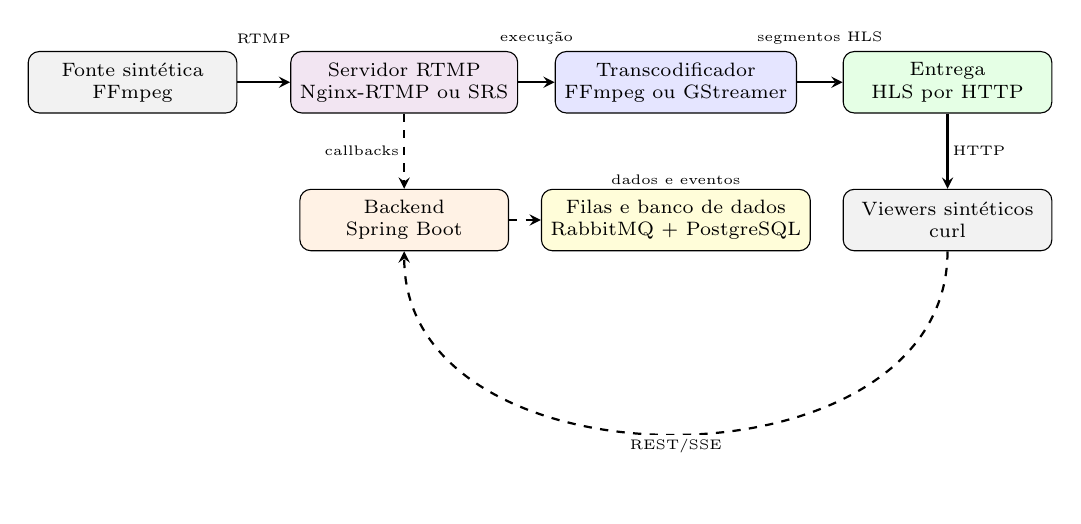
\begin{tikzpicture}[
  box/.style={draw, rounded corners, align=center, minimum width=2.65cm, minimum height=0.78cm, font=\scriptsize},
  arrow/.style={->, thick, >=stealth},
  label/.style={font=\tiny, fill=white, inner sep=1.5pt}
]
\node[box, fill=gray!10] (obs) at (0,0) {Fonte sintética\\FFmpeg};
\node[box, fill=violet!10] (rtmp) at (3.45,0) {Servidor RTMP\\Nginx-RTMP ou SRS};
\node[box, fill=blue!10] (trans) at (6.90,0) {Transcodificador\\FFmpeg ou GStreamer};
\node[box, fill=green!10] (hls) at (10.35,0) {Entrega\\HLS por HTTP};
\node[box, fill=orange!10] (backend) at (3.45,-1.75) {Backend\\Spring Boot};
\node[box, fill=yellow!15] (services) at (6.90,-1.75) {Filas e banco de dados\\RabbitMQ + PostgreSQL};
\node[box, fill=gray!10] (viewer) at (10.35,-1.75) {Viewers sintéticos\\curl};
\draw[arrow] (obs.east) -- node[above=0.42cm,label]{RTMP} (rtmp.west);
\draw[arrow] (rtmp.east) -- node[above=0.42cm,label]{execução} (trans.west);
\draw[arrow] (trans.east) -- node[above=0.42cm,label]{segmentos HLS} (hls.west);
\draw[arrow] (hls.south) -- node[right,label]{HTTP} (viewer.north);
\draw[arrow,dashed] (rtmp.south) -- node[left,label]{callbacks} (backend.north);
\draw[arrow,dashed] (backend.east) -- (services.west);
\node[anchor=south, label] at (services.north) {dados e eventos};
\draw[arrow,dashed] (viewer.south) to[out=270,in=270,looseness=1.15] node[below,label]{REST/SSE} (backend.south);
\end{tikzpicture}
\caption{Arquitetura experimental da plataforma.}
\end{figure}

\subsection{Interface da plataforma}

Além da infraestrutura de processamento, a plataforma possui uma interface web para criação de transmissões, consulta das lives disponíveis e acesso ao painel do publicador. A interface não é utilizada como instrumento primário de medição, mas demonstra o fluxo de uso que conecta a implementação experimental ao cenário de aplicação. O publicador cria uma transmissão, recebe os dados necessários para configurar o software de captura e acompanha o estado da sessão; o espectador acessa a transmissão pela página de reprodução.

\begin{figure}[H]
\centering
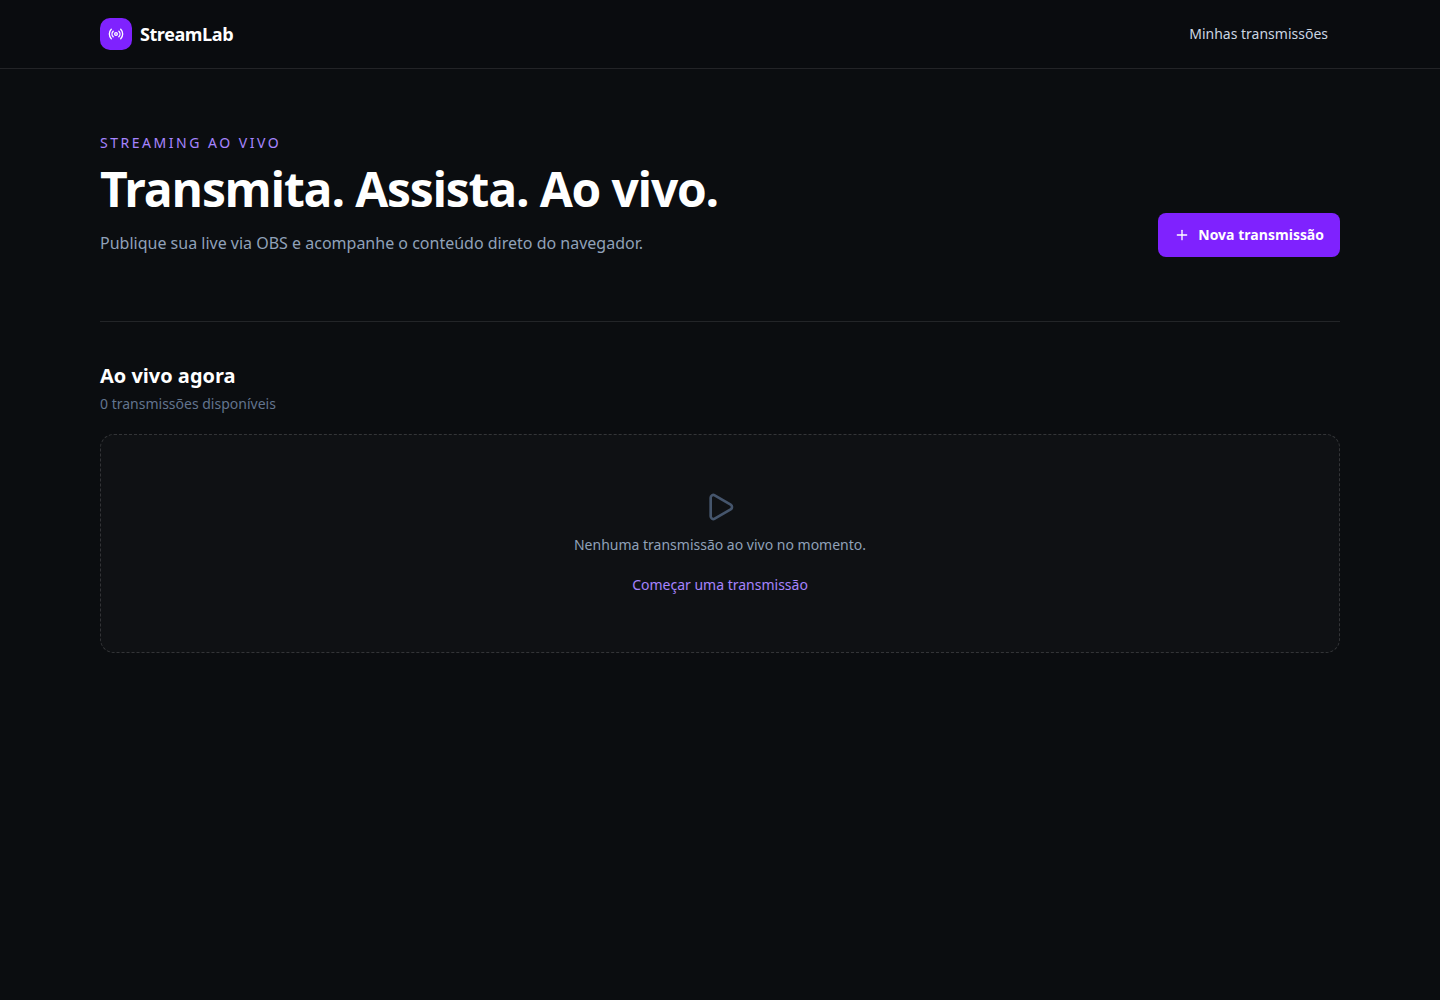
\includegraphics[width=0.94\textwidth]{../screenshots/home.png}
\caption{Tela inicial da plataforma de streaming.}
\label{fig:interface-home}
\end{figure}

A Figura~\ref{fig:interface-home} apresenta a tela inicial em seu estado sem transmissões ativas. A interface documenta a aplicação construída, mas não é usada como instrumento primário do benchmark. Dessa forma, os resultados quantitativos são produzidos pelos scripts automatizados, enquanto a figura evidencia a integração entre a infraestrutura avaliada e o cenário de uso da plataforma.

\subsection{Configuração do conteúdo e dos pipelines}

O FFmpeg gera quatro variantes (1080p, 720p, 480p e 360p) por meio de divisão do vídeo, redimensionamento, codificação H.264 e mux HLS \citep{ffmpeg}. Os alvos de vídeo são, respectivamente, 5000, 2800, 1400 e 800 kbps, com áudio de 128, 128, 96 e 96 kbps. O GStreamer executa quatro pipelines paralelos com \texttt{rtmpsrc}, decodificação, redimensionamento, \texttt{x264enc}, codificação AAC e \texttt{hlssink2} \citep{gstreamer,gstreamerhls}; seus alvos de vídeo são 5000, 2500, 1400 e 600 kbps, com os mesmos alvos de áudio. Portanto, os alvos agregados não são idênticos: aproximadamente 10,0 Mbps de vídeo no FFmpeg e 9,5 Mbps no GStreamer. Essa diferença é registrada como uma ameaça à comparabilidade e impede interpretar o bitrate como uma medida isolada de eficiência ou qualidade.

Em ambos os pipelines, a duração nominal dos segmentos HLS é de 6 segundos e a playlist mantém 10 segmentos. A codificação é realizada em CPU, sem aceleração por GPU. As quatro representações seguem o modelo de múltiplas qualidades do HLS, mas a ausência de uma normalização completa dos parâmetros significa que a comparação é entre as configurações implementadas no projeto.

\subsection{Métricas}

\begin{table}[H]
\centering
\caption{Métricas coletadas e interpretação}
\begin{tabularx}{\textwidth}{@{}lXX@{}}
\toprule
Métrica & Unidade & Definição operacional \\
\midrule
Startup da playlist mestre & s & Tempo até a playlist mestre responder HTTP 200 \\
CPU média/máxima & \% & Uso agregado do container RTMP durante a janela medida \\
Memória média/máxima & MB & Memória observada no container \\
Bitrate efetivo & kbps & Estimativa a partir dos segmentos HLS \\
Taxa de erros HTTP & \% & Requisições de playlist ou segmento com erro divididas pelo total \\
Reinícios & contagem & Diferença do contador de reinícios do container \\
Primeiro segmento / proxy E2E & s & Campo coletado, mas não validado por timestamps sincronizados \\
\bottomrule
\end{tabularx}
\end{table}

\subsection{Procedimento e análise}

Cada cenário derruba a execução anterior e sobe uma instância limpa do ambiente conteinerizado, cuja finalidade é isolar e reproduzir os serviços da aplicação \citep{docker}. Em seguida, cria-se uma transmissão, inicia-se a fonte sintética, mede-se o tempo até a playlist mestre responder, inicia-se a quantidade definida de viewers e coleta-se o estado do container com \texttt{docker stats} em intervalos de dois segundos. A sessão nominal dura 300 segundos. Os dados brutos são consolidados por uma rotina de agregação estatística, que calcula médias e desvios padrão agrupados por servidor, transcodificador e carga.

Os critérios operacionais adotados no benchmark são disponibilidade da playlist mestre em até 24 s, CPU média de até 240\% para 1 e 10 viewers e 280\% para 50 viewers, taxa de erros de até 1\% para 1 e 10 viewers e 3\% para 50 viewers, além de zero reinícios. Esses limites são critérios de aceitação do experimento local, não requisitos universais de streaming. O percentual de CPU é agregado pelo Docker e pode ultrapassar 100\% quando o processo utiliza múltiplas threads do host.

\subsection{Delineamento fatorial}

O experimento pode ser representado como um delineamento fatorial $2\times2\times3$. Os dois primeiros fatores são tecnológicos e o terceiro representa a carga. Essa organização permite observar tanto o efeito isolado de cada fator quanto a interação entre servidor e transcodificador. Por exemplo, um transcodificador pode apresentar determinado consumo quando associado ao Nginx e comportamento diferente quando associado ao SRS, ainda que a carga permaneça constante.

Para cada tratamento, as três repetições são executadas com a mesma configuração de entrada e duração nominal. A média representa o comportamento central, enquanto o desvio padrão indica a variação entre repetições. Como o número de repetições é pequeno, os desvios são usados de forma descritiva; não se pretende realizar inferência estatística forte ou atribuir significância causal às diferenças observadas.

\subsection{Controle de variáveis}

Foram mantidos constantes o host, o sistema operacional, o mecanismo de virtualização, a resolução da fonte sintética, a duração dos segmentos e os parâmetros de retenção da playlist. A variável independente principal é a combinação servidor--transcodificador; o número de espectadores funciona como fator de pressão. Como variáveis dependentes, foram observados o startup HLS, o uso de CPU e memória, o bitrate efetivo, a taxa de erros e os reinícios.

Essa separação é importante porque o bitrate produzido não deve ser interpretado isoladamente como indicador de eficiência. Ele também depende do número de variantes, das resoluções, dos bitrates-alvo e dos parâmetros do encoder. Assim, a comparação de consumo precisa ser lida junto com a configuração de saída e com a estabilidade da entrega.

\subsection{Ambiente experimental}

\begin{table}[H]
\centering
\caption{Características do ambiente experimental}
\begin{tabularx}{\textwidth}{@{}lX@{}}
\toprule
Componente & Configuração \\
\midrule
Sistema operacional & Ubuntu 24.04.3 LTS, arquitetura x86\_64 \\
Processador & Intel Core i5-13420H, 13ª geração, 12 threads \\
Memória & 24 GB de RAM \\
Armazenamento & SSD NVMe, aproximadamente 231 GB \\
Rede & Loopback e bridge do ambiente conteinerizado \\
Orquestração & Docker Engine e Docker Compose \\
Codificação & CPU, sem aceleração por GPU \\
\bottomrule
\end{tabularx}
\end{table}

O registro do ambiente é necessário porque os valores de CPU e memória não são propriedades isoladas dos servidores ou transcodificadores. O percentual de CPU observado no container pode ultrapassar 100\% quando mais de uma thread é utilizada, enquanto a memória deve ser interpretada em relação à capacidade total do host e aos demais serviços ativos. Essa preocupação é consistente com estudos de avaliação de containers, que tratam a infraestrutura e o tipo de carga como fatores inseparáveis da medição de desempenho \citep{shirinbab}.

\subsection{Reprodutibilidade}

Uma execução pode ser reproduzida seguindo a sequência de selecionar o perfil do servidor, selecionar o transcodificador, reconstruir os containers, criar a transmissão, iniciar a fonte sintética, aplicar a carga de viewers, coletar as séries temporais e repetir o tratamento. O benchmark mantém CSV bruto, logs por cenário, amostras de métricas e um CSV agregado. A execução analisada foi identificada pelo run id \texttt{bench-full-20260517-164317}; o estado do host e os parâmetros do pipeline devem ser mantidos junto desses artefatos para permitir auditoria.

\subsection{Validade e limitações}

Os resultados são internos ao host Ubuntu 24.04.3, Intel Core i5-13420H, 24 GB de RAM, SSD NVMe e Docker Engine. Não há rede externa, GPU, variação de codec, variação de resolução de entrada ou comparação com outros hosts. A latência ponta a ponta não foi instrumentada de forma válida: o script reutiliza a medição de primeiro segmento como proxy e os registros apresentam zeros na maior parte dos tratamentos. A playlist mestre responder não significa necessariamente que um segmento válido já esteja disponível nem que o player tenha iniciado a reprodução. Por isso, essa métrica não é usada como evidência conclusiva; trabalhos futuros deverão sincronizar timestamps entre publicação, criação do segmento, disponibilização HTTP e leitura pelo viewer.
